\section{Conformal Invariance}
\label{ch:conf}

In Section~\ref{sec:scaling} we talked about the principle of scale invariance
and how incredibly useful it is. It is based on the fact that the correlation
functions transform covariantly under a change in scale $\mathbf{r}\rightarrow
b\mathbf{r}$. A \textit{global} change in scale, that is. One could perfectly
construct a transformation in which the scaling factor $b$ depends on the
position $b=b(\mathbf{r})$. This would be a \textit{local} change of scale.
This kind of transformation would deform the overall shape of the system, but
in the direct vicinity of a point it would look like a regular scale
transformation with possibly a rotation and translation. Surely we don't expect
every functional form of $b(\mathbf{r})$ to behave like that, some of them
would deform the geometry of the system even at the very small scales, so we
must be careful when trying to generalize scale invariance. Luckily there
is a class of functions that look like exactly what we want, these are called
\textit{conformal transformations} or \textit{conformal maps}.

A transformation $\mathbf{r}\rightarrow\mathbf{r}'$ is conformal when it
preserve the angle between any two vectors, that is
\begin{equation}
    \theta=
    \arccos\frac{\mathbf{r}_{1}\cdot\mathbf{r}_{2}}
                {\left|\mathbf{r}_{1}\right|\left|\mathbf{r}_{2}\right|}=
    \arccos\frac{\mathbf{r}'_{1}\cdot\mathbf{r}'_{2}}
                {\left|\mathbf{r}'_{1}\right|\left|\mathbf{r}'_{2}\right|}=
    \theta'.
\end{equation}
More formally, they are coordinate changes that that keep the metric invariant
up to a local scaling factor
\begin{equation}
    g_{\mu\nu}'\left(\mathbf{r}'\right)=
    \Omega\left(\mathbf{r}\right)g_{\mu\nu}\left(\mathbf{r}\right).
\end{equation}
Figure~\ref{fig:lenna} illustrate the fact the conformal transformations do not
deform small images, it can only scale, translate or rotate them. Because of
that, translational, rotational, and scaling invariance are obvious properties
a system must have in order to be conformally invariant, another important
ingredient is locality, that is, the presence of short range interactions.
That's because if different parts of the system will be rescaled by different
factors, they must not exert direct influence over one another (they can exert
\textit{indirect} influence through long range correlations though). The recipe
for conformal invariance is, as Cardy~\cite{Domb1972} puts it
\begin{equation*}
    \left.
        \begin{array}{l}
            \mbox{Scale Invariance}\\
            \begin{array}{cl}
                + & \mbox{Translation Invariance}\\
                + & \mbox{Rotational Invariance}\\
                + & \mbox{Short-range Interactions}
            \end{array}
        \end{array}
    \right\} \Rightarrow\mbox{Conformal Invariance}.
\end{equation*}
If any of these criteria is not met, conformal invariance breaks down, which is
the case of non-local models like the Minimum Spanning Tree (given a fully
connected graph with randomly weighted edges, the minimum spanning tree is a
loopless sub-graph that connects all vertices while minimizing the sum of the
weights)~\cite{Wilson2004}.

We can implement the idea of conformal invariance in a similar way we did
for scale invariance in Eqs.~\ref{eq:scal} and~\ref{eq:scal10}.
This way, the $n$-point correlation function of any set of field
operators $\{\phi_i\}$ transforms as follows
\begin{equation}
    \left\langle
        \phi_{1}\left(\mathbf{r}_{1}\right)
        \phi_{2}\left(\mathbf{r}_{2}\right)
        \cdots
        \phi_{N}\left(\mathbf{r}_{N}\right)
    \right\rangle =
    \prod_{i=1}^{N}J{\left(\mathbf{r}_{i}\right)}^{-x_{i}}
    \left\langle
        \phi_{1}\left(\mathbf{r}_{1}'\right)
        \phi_{2}\left(\mathbf{r}_{2}'\right)
        \cdots
        \phi_{N}\left(\mathbf{r}_{N}'\right)
    \right\rangle,
\end{equation}
where in this case $J$ stands for the Jacobian of the transformation
$J{\left(\mathbf{r}\right)}^{d}=
\det\left(\partial\mathbf{r}/\partial\mathbf{r}'\right)$, and the $x_i$ are the
scaling dimension of each operator.

In $d>2$ the group of conformal transformations is finite dimensional, and
it is composed of only translations, rotations, dilations and the special
transformation
\begin{equation}
    \mathbf{r}\rightarrow\mathbf{r}'=
    \frac{\mathbf{r}+\mathbf{a}r^{2}}{1+2\mathbf{a}\cdot\mathbf{r}+a^{2}r^{2}}.
\end{equation}
These maps are known as projective conformal transformations, and are capable
of completely determining 2-point and 3-point correlation functions.
Higher order correlators cannot be determined using conformal invariance.

In $d=2$, however, the conformal group is infinite dimensional and homeomorphic
to the set of analytical functions.

Since analytical functions live and thrive in the complex plane, it is common
to work
\begin{equation}
    \begin{array}{cc}
        z=x+iy, & \bar{z}=x-iy
    \end{array}
\end{equation}

These four transformations can be condensed into one in the complex plane
\begin{equation}
    w\left(z\right)=\frac{az+b}{cz+d},\;\;\;\;\;\;\;\; ad-bc=1.
\end{equation}
Unfortunately the projective transformations are not enough to determine the 

The stress-energy tensor transforms as
\begin{equation}
    \left\langle T\left(z_{1}\right)T\left(z_{2}\right)\right\rangle=
    \frac{c/2}{{\left(z_{1}-z_{2}\right)}^{4}},
\end{equation}
which define the \textit{central charge} $c$.

Conformal invariance ha


\begin{figure}
\begin{center}
    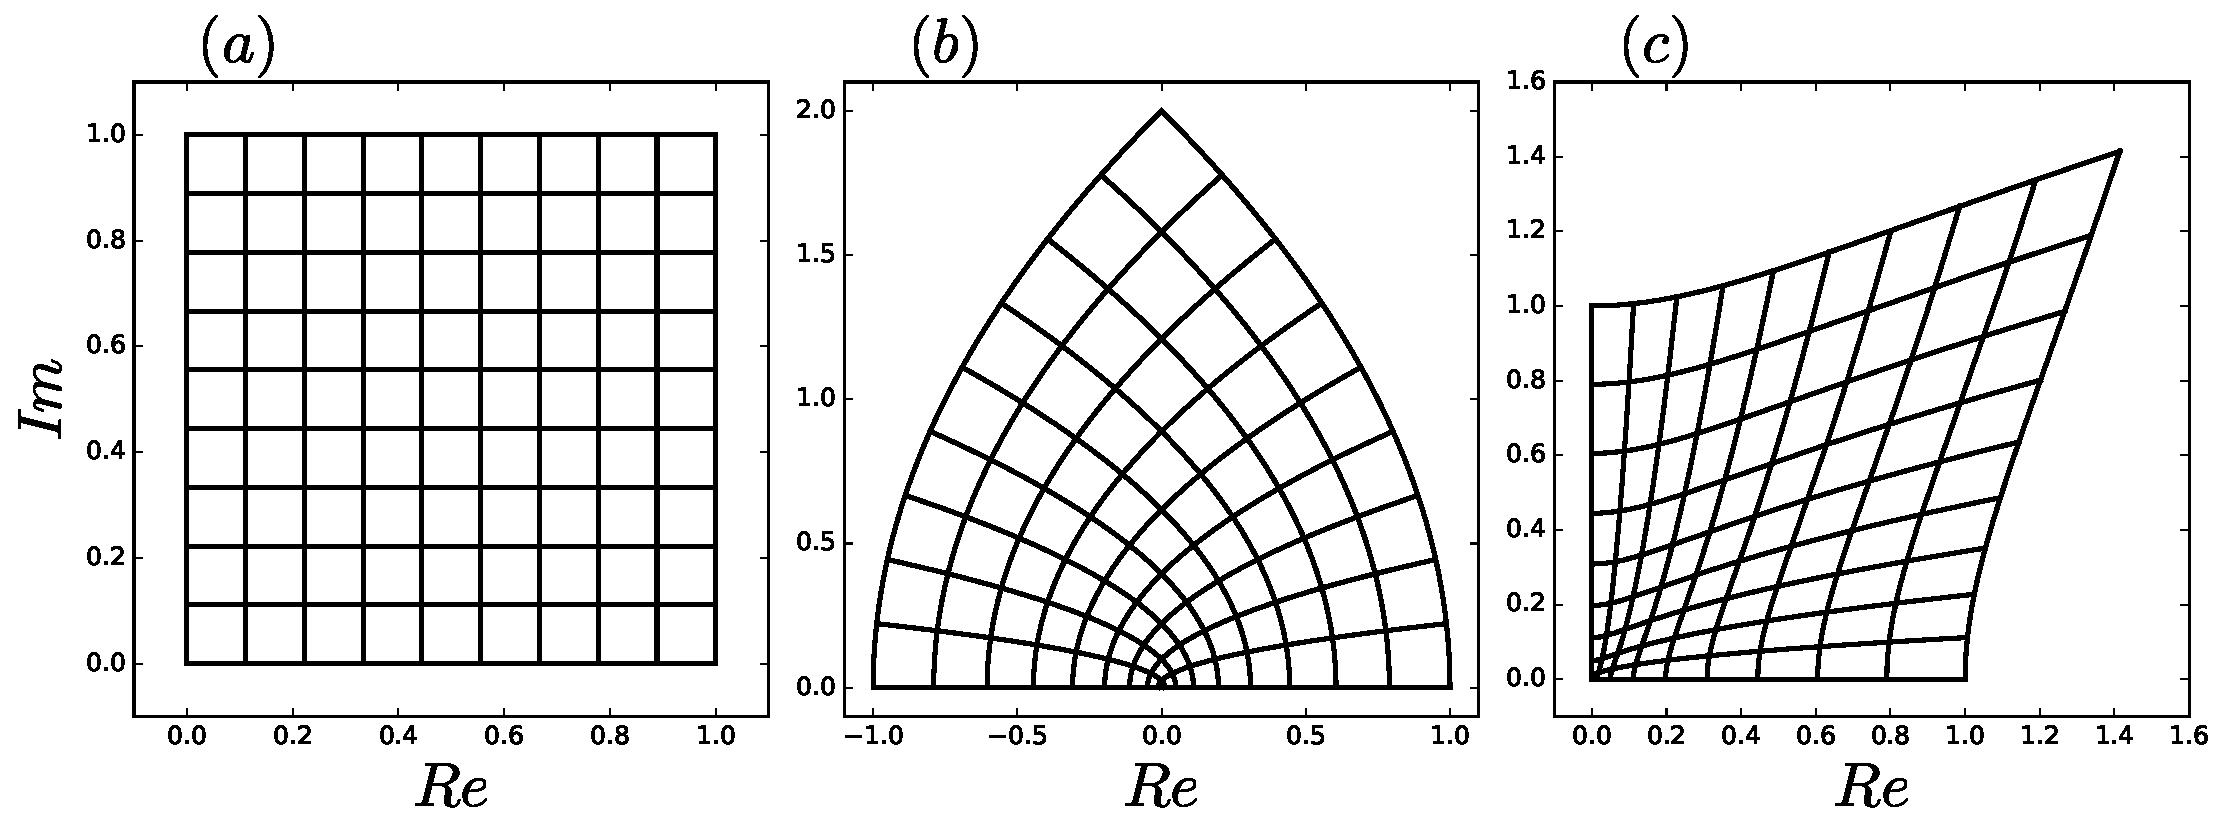
\includegraphics[width=\textwidth]{chapters/ch3-conf/figs/cmapex}
\end{center}
\caption{Coordinates transformations in the complex plane can be divided into
    conformal and non-conformal. Conformal transformations preserve the
    intersection angles between lines, unlike the non-conformal. The
    transformation from the square lattice in (a) into (b) is conformal
    ($f(z)=z^2$), while the one from (a) to (c) ($f(z)=z|z|$) is not.}
\label{fig:cmapex}
\end{figure}

\begin{figure}
\begin{center}
    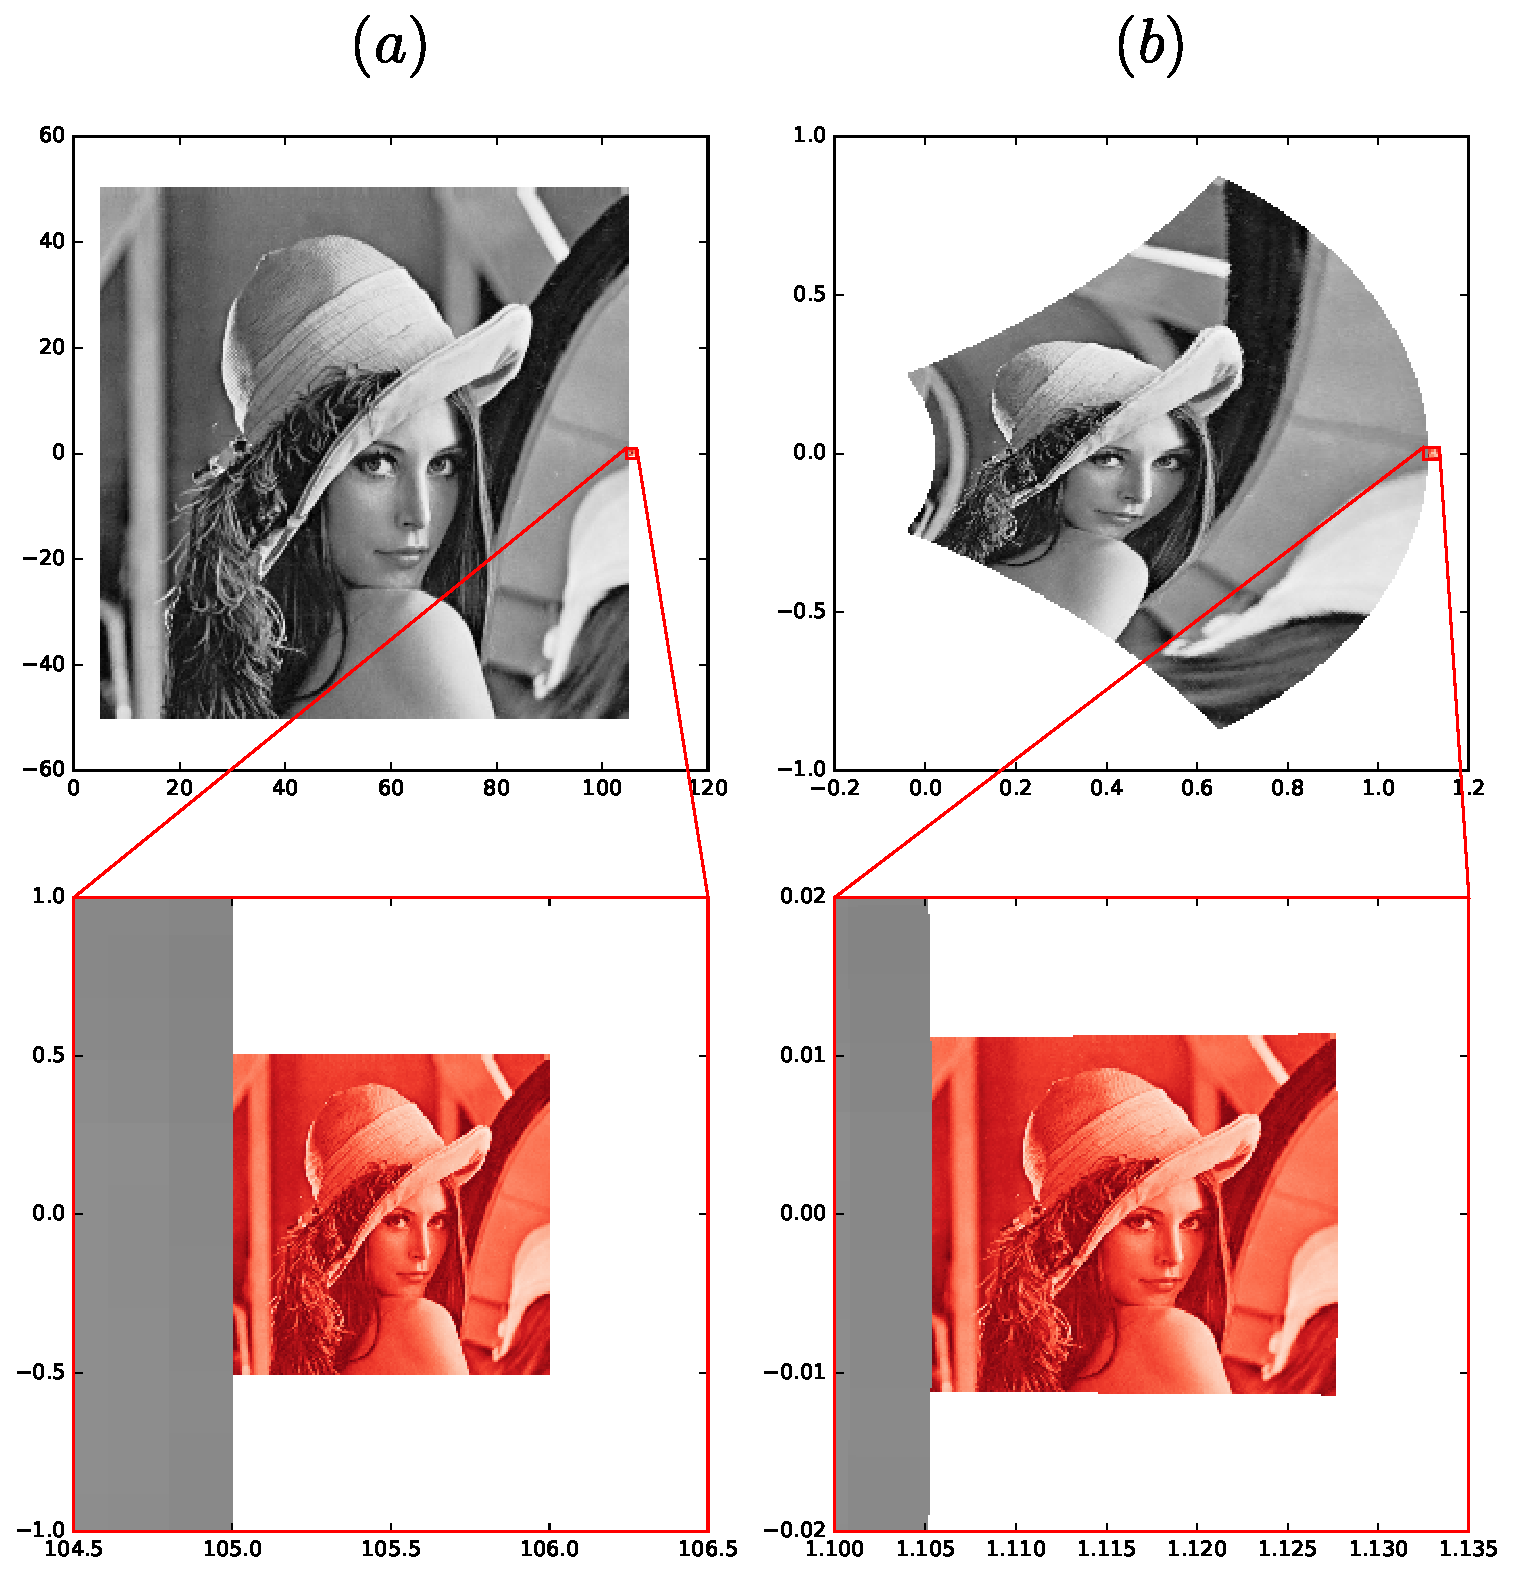
\includegraphics[width=0.66\textwidth]{chapters/ch3-conf/figs/lenna}
\end{center}
\caption{Two identical images, one large (in grayscale) and the other small (in
    red, shown in the zoom), are transformed from (a) to (b) using a conformal
    map $f(z)=z/(200-z)$. While the large one is heavily deformed, the smaller
    one was only translated and shrunk. This illustrates the fact that conformal
    maps behave locally as a scale transformation.}
\label{fig:lenna}
\end{figure}



\begin{figure}
\begin{center}
    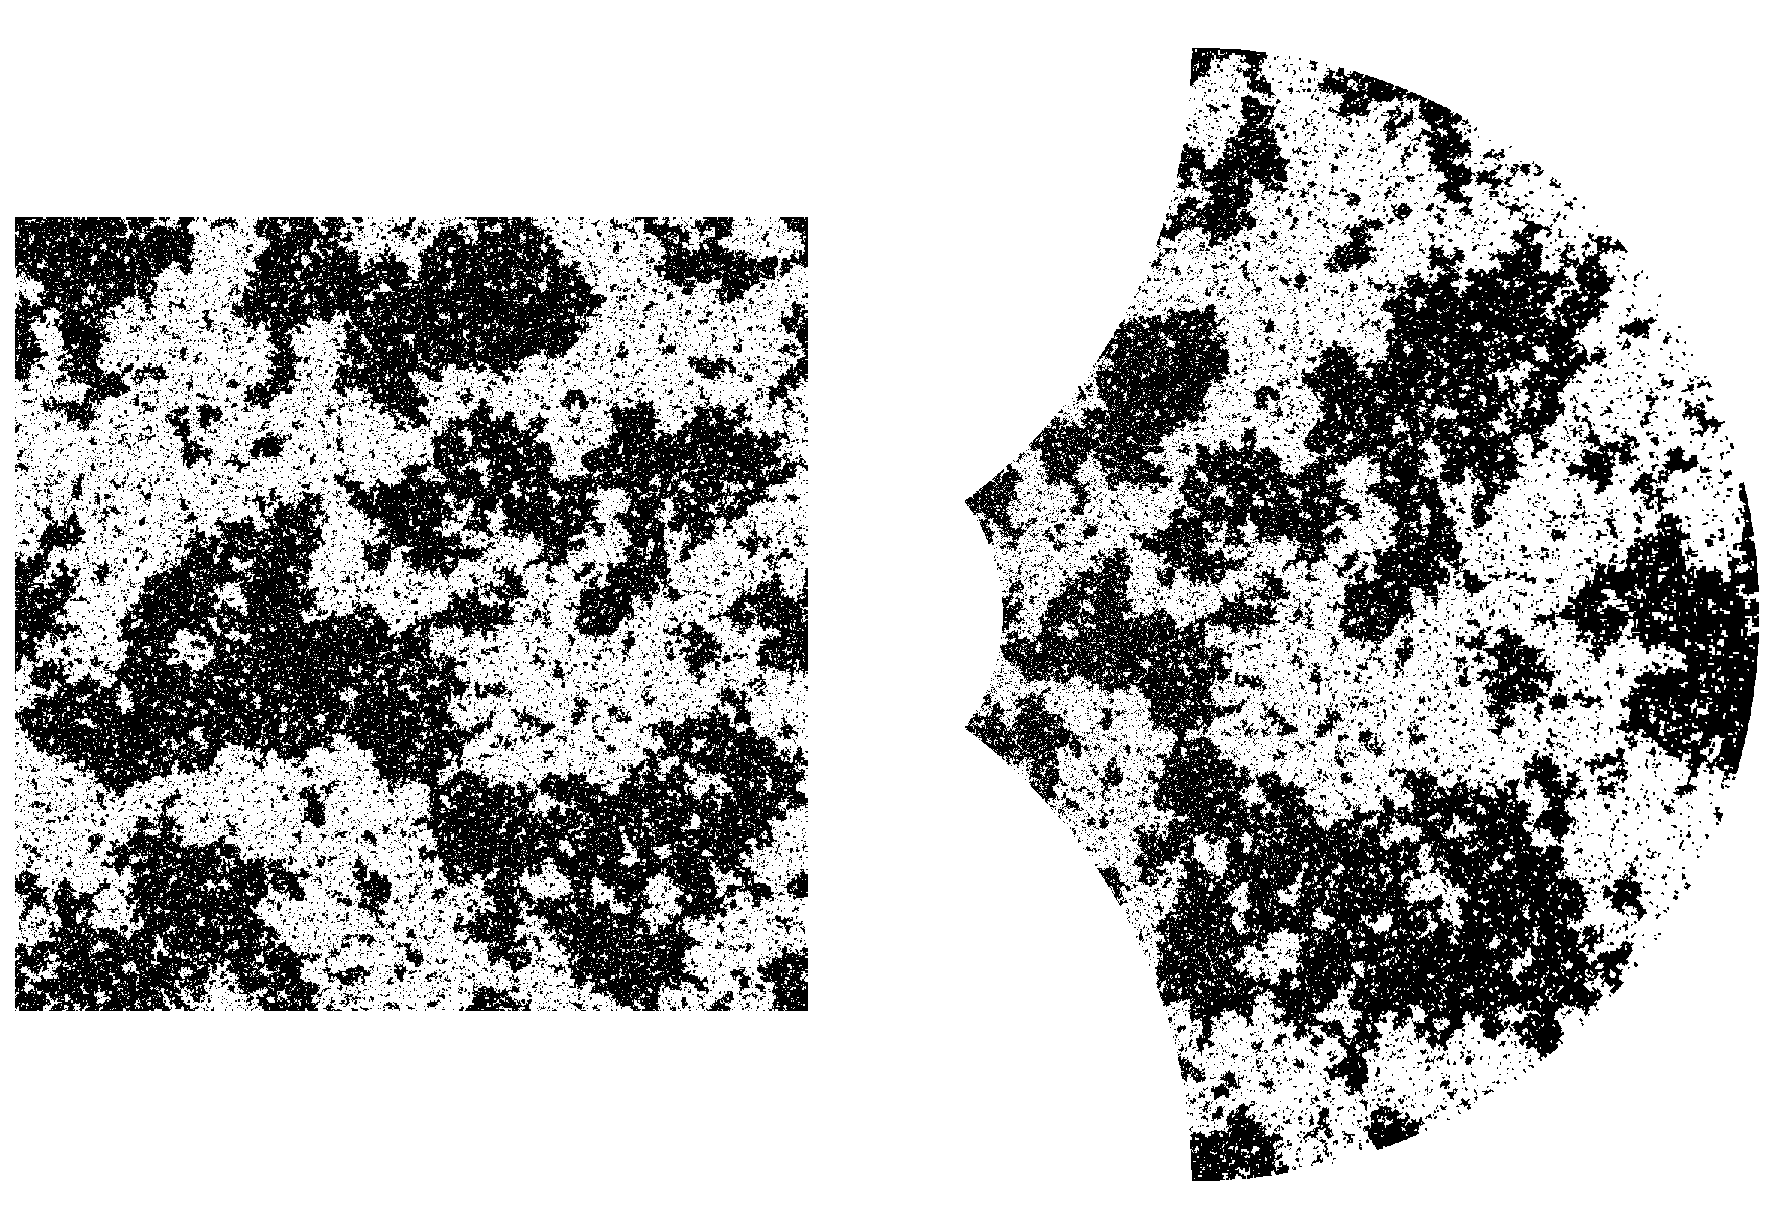
\includegraphics[width=0.8\textwidth]{chapters/ch3-conf/figs/isingcm}
\end{center}
\caption{Illustration of the Ising model at the critical point when transformed
    under a conformal map $f(z)=z/(2-z)$. The deformed image still looks
    statistically similar to the original, which is a consequence of conformal
    invariance.}
\label{fig:isingcm}
\end{figure}

\begin{figure}
\begin{center}
    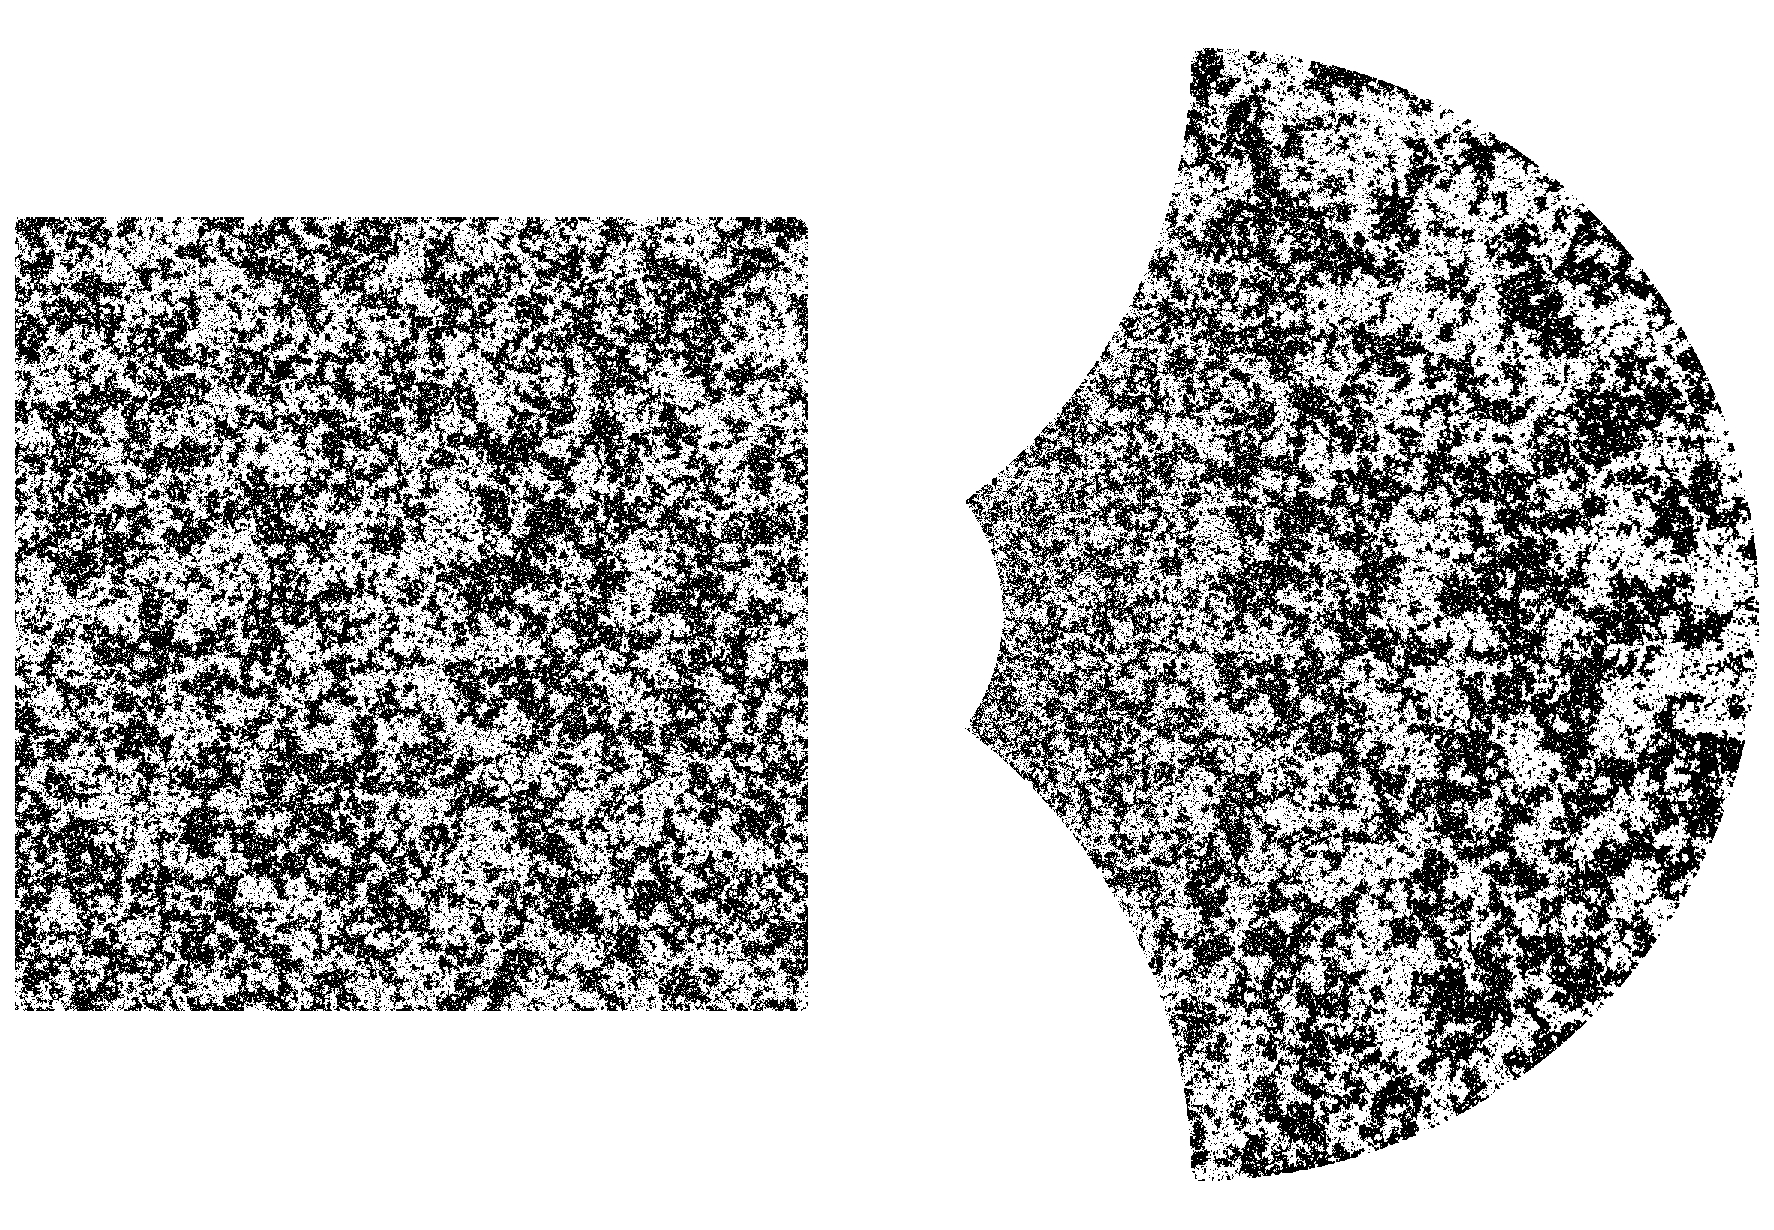
\includegraphics[width=0.8\textwidth]{chapters/ch3-conf/figs/isingcm2}
\end{center}
\caption{Illustration of the Ising model above the critical point when
    transformed under a conformal map $f(z)=z/(2-z)$. In the deformed image,
    the spin configuration is no longer homogeneous, because outside the
    critical point the system is no longer conformally invariant.}
\label{fig:isingcm2}
\end{figure}
